\section{Sketch of approach\hfill\textnormal{\emph{Löbel}}}
Nach Festlegung der funktionalen Anforderungen wurde ein erster Prototyp im 3D erstellt. Grundlage hierfür waren einzelene Paper Prototypes der Gruppenmitglieder. Nach Bewertung der einzelnen Prototypes wurden Teile bzw. Komponenten übernommen oder ergänzt. 


\subsection{3D Prototype}
Der resultierende Prototype, siehe Abb.\ref{fig:model_proto}, beinhaltete wie in den Anforderungen bereits erwähnt, einen Kettenantrieb für die Fortbewegung an Land. Für die Fortbewegung im Wasser wurden Turbine und Ruder zentral im unteren Bereich des Roboters in einem Durchgangsloch platziert. Für das Bergen von Gegenständen wurde ein schwenkbarer Greifarm mit Greifer zentral an der Fahrzeug Vorderseite positioniert. Der Greifer wurde von der GrabCAD Library importiert, \textit{\url{https://grabcad.com/library/4-bar-linkage-gripper-with-dynamixel-rx-64-1}}. Zur zusätzlichen Unterstützung beim Greifprozess wurden im Prototype zwei heraus fahrbare Stützen an Fahrzeug Vorderseite angebracht. Zum Sammeln der radioaktiven Gegenstände befindet sich im hinteren Teil des Roboters eine verschließbare Box. Daneben wurde eine offene Box eingebracht zum Laden von beispielsweise "Erste-Hilfe" Material oder einem Koffer. Vorne links am Fahrzeug wurden LIDAR Sensor inklusive Peripherie wie Kamera, Lautsprecher und Mikrophon auf einem Drehpodest platziert. Zusätzlich ist dieser Teil schwenkbar.

\begin{figure}[H]
  \centering{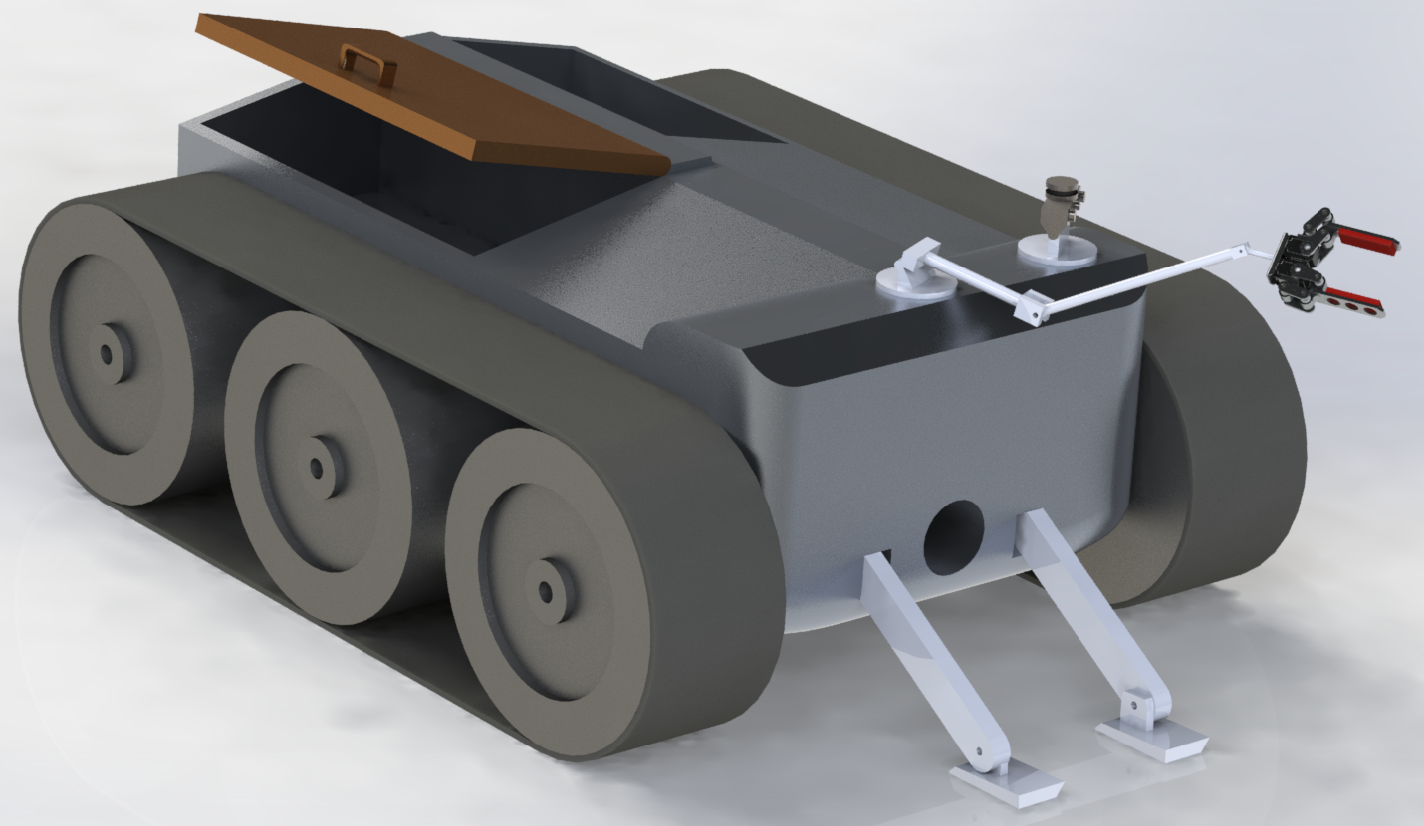
\includegraphics[width=1.0\linewidth]{Abbildungen/3D_model/prototype_front.png}}
  \caption{Kombinierter 3D Prototyp}
  \label{fig:model_proto}
\end{figure}